\batchmode
\documentclass[a4paper]{book}
\usepackage{makeidx}
\usepackage{natbib}
\usepackage{graphicx}
\usepackage{multicol}
\usepackage{float}
\usepackage{listings}
\usepackage{color}
\usepackage{ifthen}
\usepackage[table]{xcolor}
\usepackage{textcomp}
\usepackage{alltt}
\usepackage[utf8]{inputenc}
\usepackage{mathptmx}
\usepackage[scaled=.90]{helvet}
\usepackage{courier}
\usepackage{sectsty}
\usepackage[titles]{tocloft}
\usepackage{doxygen}
\lstset{language=C++,inputencoding=utf8,basicstyle=\footnotesize,breaklines=true,breakatwhitespace=true,tabsize=8,numbers=left }
\makeindex
\setcounter{tocdepth}{3}
\renewcommand{\footrulewidth}{0.4pt}
\renewcommand{\familydefault}{\sfdefault}
\hfuzz=15pt
\setlength{\emergencystretch}{15pt}
\hbadness=750
\tolerance=750
\begin{document}
\begin{titlepage}
\vspace*{7cm}
\begin{center}
{\Large rocs\-\_\-teleop }\\
\vspace*{1cm}
{\large \-Generated by Doxygen 1.7.6.1}\\
\vspace*{0.5cm}
{\small Sun Nov 11 2012 17:05:03}\\
\end{center}
\end{titlepage}
\clearemptydoublepage
\pagenumbering{roman}
\tableofcontents
\clearemptydoublepage
\pagenumbering{arabic}
\chapter{\-Main \-Page}
\label{index}

\-This package does not offer any \-C++ \-A\-P\-I. 
\chapter{\-Class \-Index}
\section{\-Class \-List}
\-Here are the classes, structs, unions and interfaces with brief descriptions\-:\begin{DoxyCompactList}
\item\contentsline{section}{{\bf \-Turtlebot\-Teleop} }{\pageref{classTurtlebotTeleop}}{}
\end{DoxyCompactList}

\chapter{\-File \-Index}
\section{\-File \-List}
\-Here is a list of all files with brief descriptions\-:\begin{DoxyCompactList}
\item\contentsline{section}{{\bf joy.\-cpp} }{\pageref{joy_8cpp}}{}
\end{DoxyCompactList}

\chapter{\-Class \-Documentation}
\section{\-Turtlebot\-Teleop \-Class \-Reference}
\label{classTurtlebotTeleop}\index{\-Turtlebot\-Teleop@{\-Turtlebot\-Teleop}}
\subsection*{\-Public \-Member \-Functions}
\begin{DoxyCompactItemize}
\item 
{\bf \-Turtlebot\-Teleop} ()
\end{DoxyCompactItemize}
\subsection*{\-Private \-Member \-Functions}
\begin{DoxyCompactItemize}
\item 
void {\bf joy\-Callback} (const sensor\-\_\-msgs\-::\-Joy\-::\-Const\-Ptr \&joy)
\item 
void {\bf publish} ()
\end{DoxyCompactItemize}
\subsection*{\-Private \-Attributes}
\begin{DoxyCompactItemize}
\item 
double {\bf a\-\_\-scale\-\_\-}
\item 
int {\bf angular\-\_\-}
\item 
int {\bf deadman\-\_\-axis\-\_\-}
\item 
bool {\bf deadman\-\_\-pressed\-\_\-}
\item 
ros\-::\-Subscriber {\bf joy\-\_\-sub\-\_\-}
\item 
double {\bf l\-\_\-scale\-\_\-}
\item 
geometry\-\_\-msgs\-::\-Twist {\bf last\-\_\-published\-\_\-}
\item 
int {\bf linear\-\_\-}
\item 
ros\-::\-Node\-Handle {\bf nh\-\_\-}
\item 
ros\-::\-Node\-Handle {\bf ph\-\_\-}
\item 
boost\-::mutex {\bf publish\-\_\-mutex\-\_\-}
\item 
ros\-::\-Timer {\bf timer\-\_\-}
\item 
ros\-::\-Publisher {\bf vel\-\_\-pub\-\_\-}
\end{DoxyCompactItemize}


\subsection{\-Detailed \-Description}


\-Definition at line 37 of file joy.\-cpp.



\subsection{\-Constructor \& \-Destructor \-Documentation}
\index{\-Turtlebot\-Teleop@{\-Turtlebot\-Teleop}!\-Turtlebot\-Teleop@{\-Turtlebot\-Teleop}}
\index{\-Turtlebot\-Teleop@{\-Turtlebot\-Teleop}!TurtlebotTeleop@{\-Turtlebot\-Teleop}}
\subsubsection[{\-Turtlebot\-Teleop}]{\setlength{\rightskip}{0pt plus 5cm}{\bf \-Turtlebot\-Teleop\-::\-Turtlebot\-Teleop} (
\begin{DoxyParamCaption}
{}
\end{DoxyParamCaption}
)}\label{classTurtlebotTeleop_ad7b298eab45f53c4b701184fe32bf914}


\-Definition at line 60 of file joy.\-cpp.



\subsection{\-Member \-Function \-Documentation}
\index{\-Turtlebot\-Teleop@{\-Turtlebot\-Teleop}!joy\-Callback@{joy\-Callback}}
\index{joy\-Callback@{joy\-Callback}!TurtlebotTeleop@{\-Turtlebot\-Teleop}}
\subsubsection[{joy\-Callback}]{\setlength{\rightskip}{0pt plus 5cm}void {\bf \-Turtlebot\-Teleop\-::joy\-Callback} (
\begin{DoxyParamCaption}
\item[{const sensor\-\_\-msgs\-::\-Joy\-::\-Const\-Ptr \&}]{joy}
\end{DoxyParamCaption}
)\hspace{0.3cm}{\ttfamily  [private]}}\label{classTurtlebotTeleop_aa94b680ce3a5269dfe3d9d9a476e2054}


\-Definition at line 80 of file joy.\-cpp.

\index{\-Turtlebot\-Teleop@{\-Turtlebot\-Teleop}!publish@{publish}}
\index{publish@{publish}!TurtlebotTeleop@{\-Turtlebot\-Teleop}}
\subsubsection[{publish}]{\setlength{\rightskip}{0pt plus 5cm}void {\bf \-Turtlebot\-Teleop\-::publish} (
\begin{DoxyParamCaption}
{}
\end{DoxyParamCaption}
)\hspace{0.3cm}{\ttfamily  [private]}}\label{classTurtlebotTeleop_a4b7829acc3ee31188c64e979bba06c8a}


\-Definition at line 90 of file joy.\-cpp.



\subsection{\-Member \-Data \-Documentation}
\index{\-Turtlebot\-Teleop@{\-Turtlebot\-Teleop}!a\-\_\-scale\-\_\-@{a\-\_\-scale\-\_\-}}
\index{a\-\_\-scale\-\_\-@{a\-\_\-scale\-\_\-}!TurtlebotTeleop@{\-Turtlebot\-Teleop}}
\subsubsection[{a\-\_\-scale\-\_\-}]{\setlength{\rightskip}{0pt plus 5cm}double {\bf \-Turtlebot\-Teleop\-::a\-\_\-scale\-\_\-}\hspace{0.3cm}{\ttfamily  [private]}}\label{classTurtlebotTeleop_a54ffb87bd2f457ec15da5582c5c57597}


\-Definition at line 49 of file joy.\-cpp.

\index{\-Turtlebot\-Teleop@{\-Turtlebot\-Teleop}!angular\-\_\-@{angular\-\_\-}}
\index{angular\-\_\-@{angular\-\_\-}!TurtlebotTeleop@{\-Turtlebot\-Teleop}}
\subsubsection[{angular\-\_\-}]{\setlength{\rightskip}{0pt plus 5cm}int {\bf \-Turtlebot\-Teleop\-::angular\-\_\-}\hspace{0.3cm}{\ttfamily  [private]}}\label{classTurtlebotTeleop_a6ffe51200bedf54be736c7d150f1ddf5}


\-Definition at line 48 of file joy.\-cpp.

\index{\-Turtlebot\-Teleop@{\-Turtlebot\-Teleop}!deadman\-\_\-axis\-\_\-@{deadman\-\_\-axis\-\_\-}}
\index{deadman\-\_\-axis\-\_\-@{deadman\-\_\-axis\-\_\-}!TurtlebotTeleop@{\-Turtlebot\-Teleop}}
\subsubsection[{deadman\-\_\-axis\-\_\-}]{\setlength{\rightskip}{0pt plus 5cm}int {\bf \-Turtlebot\-Teleop\-::deadman\-\_\-axis\-\_\-}\hspace{0.3cm}{\ttfamily  [private]}}\label{classTurtlebotTeleop_a58071795d1025f8d5b8650e5625a47b1}


\-Definition at line 48 of file joy.\-cpp.

\index{\-Turtlebot\-Teleop@{\-Turtlebot\-Teleop}!deadman\-\_\-pressed\-\_\-@{deadman\-\_\-pressed\-\_\-}}
\index{deadman\-\_\-pressed\-\_\-@{deadman\-\_\-pressed\-\_\-}!TurtlebotTeleop@{\-Turtlebot\-Teleop}}
\subsubsection[{deadman\-\_\-pressed\-\_\-}]{\setlength{\rightskip}{0pt plus 5cm}bool {\bf \-Turtlebot\-Teleop\-::deadman\-\_\-pressed\-\_\-}\hspace{0.3cm}{\ttfamily  [private]}}\label{classTurtlebotTeleop_a343c1fd576883c946c8a106039b4f66f}


\-Definition at line 55 of file joy.\-cpp.

\index{\-Turtlebot\-Teleop@{\-Turtlebot\-Teleop}!joy\-\_\-sub\-\_\-@{joy\-\_\-sub\-\_\-}}
\index{joy\-\_\-sub\-\_\-@{joy\-\_\-sub\-\_\-}!TurtlebotTeleop@{\-Turtlebot\-Teleop}}
\subsubsection[{joy\-\_\-sub\-\_\-}]{\setlength{\rightskip}{0pt plus 5cm}ros\-::\-Subscriber {\bf \-Turtlebot\-Teleop\-::joy\-\_\-sub\-\_\-}\hspace{0.3cm}{\ttfamily  [private]}}\label{classTurtlebotTeleop_a663ab35d03be3b3f7e8d3cdea471b147}


\-Definition at line 51 of file joy.\-cpp.

\index{\-Turtlebot\-Teleop@{\-Turtlebot\-Teleop}!l\-\_\-scale\-\_\-@{l\-\_\-scale\-\_\-}}
\index{l\-\_\-scale\-\_\-@{l\-\_\-scale\-\_\-}!TurtlebotTeleop@{\-Turtlebot\-Teleop}}
\subsubsection[{l\-\_\-scale\-\_\-}]{\setlength{\rightskip}{0pt plus 5cm}double {\bf \-Turtlebot\-Teleop\-::l\-\_\-scale\-\_\-}\hspace{0.3cm}{\ttfamily  [private]}}\label{classTurtlebotTeleop_a7b259719ee155dba7ade2e7b668fbefc}


\-Definition at line 49 of file joy.\-cpp.

\index{\-Turtlebot\-Teleop@{\-Turtlebot\-Teleop}!last\-\_\-published\-\_\-@{last\-\_\-published\-\_\-}}
\index{last\-\_\-published\-\_\-@{last\-\_\-published\-\_\-}!TurtlebotTeleop@{\-Turtlebot\-Teleop}}
\subsubsection[{last\-\_\-published\-\_\-}]{\setlength{\rightskip}{0pt plus 5cm}geometry\-\_\-msgs\-::\-Twist {\bf \-Turtlebot\-Teleop\-::last\-\_\-published\-\_\-}\hspace{0.3cm}{\ttfamily  [private]}}\label{classTurtlebotTeleop_a71d2287705917566bd33239db260a680}


\-Definition at line 53 of file joy.\-cpp.

\index{\-Turtlebot\-Teleop@{\-Turtlebot\-Teleop}!linear\-\_\-@{linear\-\_\-}}
\index{linear\-\_\-@{linear\-\_\-}!TurtlebotTeleop@{\-Turtlebot\-Teleop}}
\subsubsection[{linear\-\_\-}]{\setlength{\rightskip}{0pt plus 5cm}int {\bf \-Turtlebot\-Teleop\-::linear\-\_\-}\hspace{0.3cm}{\ttfamily  [private]}}\label{classTurtlebotTeleop_a149ff3966ce0cafd27a9610e247de19e}


\-Definition at line 48 of file joy.\-cpp.

\index{\-Turtlebot\-Teleop@{\-Turtlebot\-Teleop}!nh\-\_\-@{nh\-\_\-}}
\index{nh\-\_\-@{nh\-\_\-}!TurtlebotTeleop@{\-Turtlebot\-Teleop}}
\subsubsection[{nh\-\_\-}]{\setlength{\rightskip}{0pt plus 5cm}ros\-::\-Node\-Handle {\bf \-Turtlebot\-Teleop\-::nh\-\_\-}\hspace{0.3cm}{\ttfamily  [private]}}\label{classTurtlebotTeleop_aa25e6e15a9d9a5d3b5eb135e11a888eb}


\-Definition at line 46 of file joy.\-cpp.

\index{\-Turtlebot\-Teleop@{\-Turtlebot\-Teleop}!ph\-\_\-@{ph\-\_\-}}
\index{ph\-\_\-@{ph\-\_\-}!TurtlebotTeleop@{\-Turtlebot\-Teleop}}
\subsubsection[{ph\-\_\-}]{\setlength{\rightskip}{0pt plus 5cm}ros\-::\-Node\-Handle {\bf \-Turtlebot\-Teleop\-::ph\-\_\-}\hspace{0.3cm}{\ttfamily  [private]}}\label{classTurtlebotTeleop_a966ac7baf800aa218607c7449087c16e}


\-Definition at line 46 of file joy.\-cpp.

\index{\-Turtlebot\-Teleop@{\-Turtlebot\-Teleop}!publish\-\_\-mutex\-\_\-@{publish\-\_\-mutex\-\_\-}}
\index{publish\-\_\-mutex\-\_\-@{publish\-\_\-mutex\-\_\-}!TurtlebotTeleop@{\-Turtlebot\-Teleop}}
\subsubsection[{publish\-\_\-mutex\-\_\-}]{\setlength{\rightskip}{0pt plus 5cm}boost\-::mutex {\bf \-Turtlebot\-Teleop\-::publish\-\_\-mutex\-\_\-}\hspace{0.3cm}{\ttfamily  [private]}}\label{classTurtlebotTeleop_aa9d3796c5ad60a96824ac351906ef0aa}


\-Definition at line 54 of file joy.\-cpp.

\index{\-Turtlebot\-Teleop@{\-Turtlebot\-Teleop}!timer\-\_\-@{timer\-\_\-}}
\index{timer\-\_\-@{timer\-\_\-}!TurtlebotTeleop@{\-Turtlebot\-Teleop}}
\subsubsection[{timer\-\_\-}]{\setlength{\rightskip}{0pt plus 5cm}ros\-::\-Timer {\bf \-Turtlebot\-Teleop\-::timer\-\_\-}\hspace{0.3cm}{\ttfamily  [private]}}\label{classTurtlebotTeleop_ac6f49f7a752545dfea96a6b2829bf0dc}


\-Definition at line 56 of file joy.\-cpp.

\index{\-Turtlebot\-Teleop@{\-Turtlebot\-Teleop}!vel\-\_\-pub\-\_\-@{vel\-\_\-pub\-\_\-}}
\index{vel\-\_\-pub\-\_\-@{vel\-\_\-pub\-\_\-}!TurtlebotTeleop@{\-Turtlebot\-Teleop}}
\subsubsection[{vel\-\_\-pub\-\_\-}]{\setlength{\rightskip}{0pt plus 5cm}ros\-::\-Publisher {\bf \-Turtlebot\-Teleop\-::vel\-\_\-pub\-\_\-}\hspace{0.3cm}{\ttfamily  [private]}}\label{classTurtlebotTeleop_a944ab5d8ea5a71817ac8d02ffdbc2188}


\-Definition at line 50 of file joy.\-cpp.



\-The documentation for this class was generated from the following file\-:\begin{DoxyCompactItemize}
\item 
{\bf joy.\-cpp}\end{DoxyCompactItemize}

\chapter{\-File \-Documentation}
\section{joy.\-cpp \-File \-Reference}
\label{joy_8cpp}\index{joy.\-cpp@{joy.\-cpp}}
{\ttfamily \#include $<$ros/ros.\-h$>$}\*
{\ttfamily \#include $<$geometry\-\_\-msgs/\-Twist.\-h$>$}\*
{\ttfamily \#include $<$sensor\-\_\-msgs/\-Joy.\-h$>$}\*
{\ttfamily \#include \char`\"{}boost/thread/mutex.\-hpp\char`\"{}}\*
{\ttfamily \#include \char`\"{}boost/thread/thread.\-hpp\char`\"{}}\*
{\ttfamily \#include \char`\"{}ros/console.\-h\char`\"{}}\*
\-Include dependency graph for joy.\-cpp\-:
\nopagebreak
\begin{figure}[H]
\begin{center}
\leavevmode
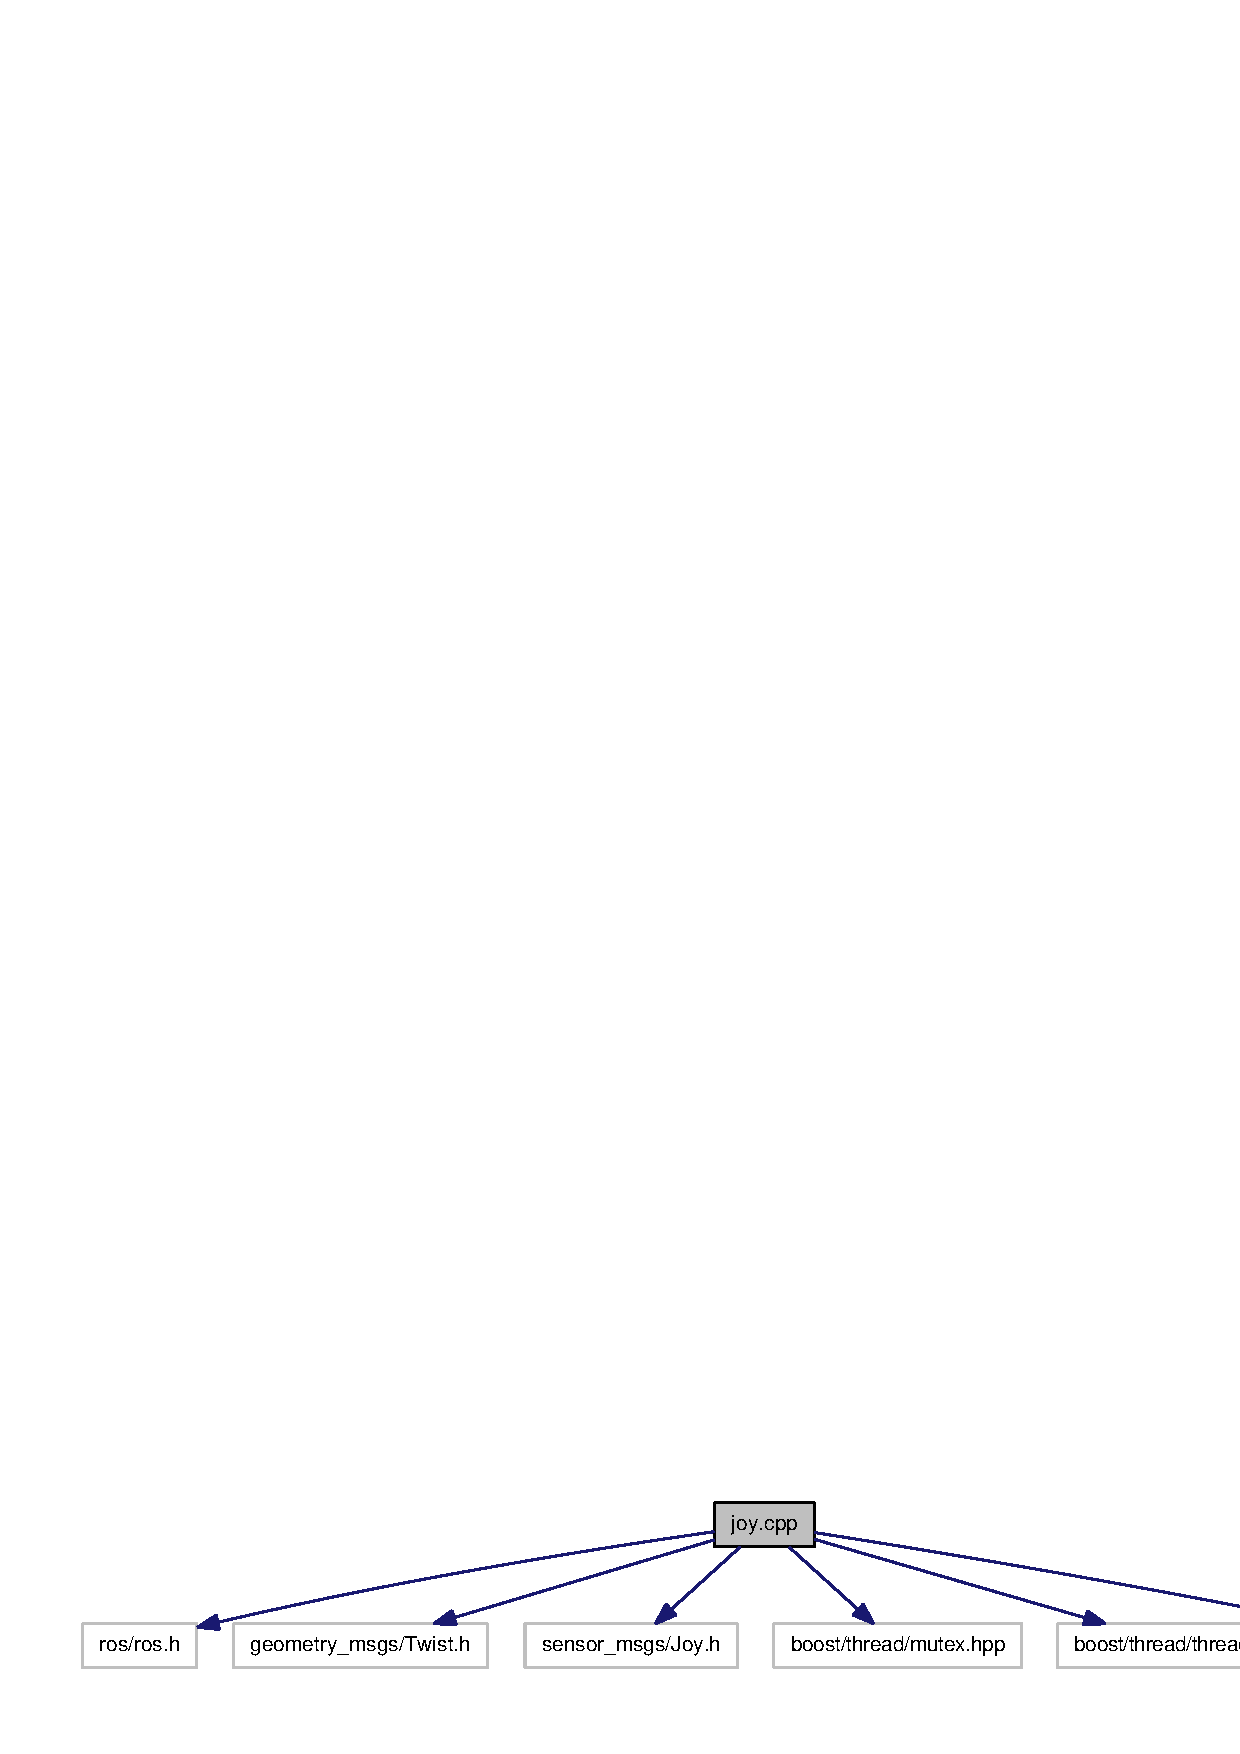
\includegraphics[width=350pt]{joy_8cpp__incl}
\end{center}
\end{figure}
\subsection*{\-Classes}
\begin{DoxyCompactItemize}
\item 
class {\bf \-Turtlebot\-Teleop}
\end{DoxyCompactItemize}
\subsection*{\-Functions}
\begin{DoxyCompactItemize}
\item 
int {\bf main} (int argc, char $\ast$$\ast$argv)
\end{DoxyCompactItemize}


\subsection{\-Function \-Documentation}
\index{joy.\-cpp@{joy.\-cpp}!main@{main}}
\index{main@{main}!joy.cpp@{joy.\-cpp}}
\subsubsection[{main}]{\setlength{\rightskip}{0pt plus 5cm}int {\bf main} (
\begin{DoxyParamCaption}
\item[{int}]{argc, }
\item[{char $\ast$$\ast$}]{argv}
\end{DoxyParamCaption}
)}\label{joy_8cpp_a3c04138a5bfe5d72780bb7e82a18e627}


\-Definition at line 100 of file joy.\-cpp.


\input{mainpage_8dox}
\printindex
\end{document}
